\documentclass{article}
\usepackage{graphicx} % Required for inserting images
\usepackage{listings}
\usepackage{xcolor}
\usepackage{tikz}
\usepackage{hyperref}
\usepackage{geometry}
\usepackage{listings}
\usepackage{amsmath}
\usetikzlibrary {automata,positioning}
\definecolor{codegreen}{rgb}{0,0.6,0}
\definecolor{codegray}{rgb}{0.5,0.5,0.5}
\definecolor{codepurple}{rgb}{0.58,0,0.82}
\definecolor{backcolour}{rgb}{0.95,0.95,0.92}
\lstdefinestyle{mystyle}{
    backgroundcolor=\color{backcolour},
    commentstyle=\color{codegreen},
    keywordstyle=\color{magenta},
    numberstyle=\tiny\color{codegray},
    stringstyle=\color{codepurple},
    basicstyle=\ttfamily\scriptsize,
    breakatwhitespace=false,
    breaklines=true,
    captionpos=b,
    keepspaces=true,
    numbers=left,
    numbersep=1pt,
    showspaces=false,
    showstringspaces=false,
    showtabs=false,
    tabsize=2,
    inputencoding=utf8,
    extendedchars=true,
}
%\lstset{language=Haskell}
\lstset{style=mystyle}
\setlength{\parindent}{0in}

\title{24-11-2024}
\author{Samuel Fournier}
\date{November 2024}

\begin{document}

\maketitle

Dans le dernier mois (oui, ça fait déjà un mois depuis le dernier rapport). J'ai continuer de travailler sur le \textit{Ray Marching}. Malheureusement, lors de mon implémentation initiale de l'algorithme, j'ai commis certaines erreurs. La première et la plus importante selon moi, était le calcul de la couleur de scatter. Dans la première itération du code, la couleur du scatter finissait toujours par être \textbf{(0,0,0)}, ce qui faisait en sorte que la couleur finale n'était que la couleur de l'objet multiplié par le facteur d'opacité \textbf{hit.transmittance}. De se fait, la fumée résultante était très sombre (presque noir) dans les régions où la densité était élevé. La raison pour le problème était à cause de cette ligne de code dans la fonction \textbf{lightMediumIntersection}:
\begin{lstlisting}[language=C++]
    if ((tmin > tymax) || (tymin > tmax)) return false;
\end{lstlisting}
Lorsque j'ai écrit cette fonction, je n'ai que copié la fonction d'intersection avec le médium \textbf{localIntersect}, cependant cette fonction ne gère pas le cas où l'origine du rayon est à l'intérieur du médium. Lorsque l'on tire le \textbf{lightRay}, son origine est à l'intérieur du médium, ce qui fait en sorte que l'on entre dans ce \textbf{if} et on retourne \textbf{false}. Ensuite, on utilise cette valeur de retour pour tester:
\begin{lstlisting}[language=C++]
    // Use epsilon to avoid self intersection;
    if(!lightMediumIntersection(lightRay, EPSILON, &t_light)) {
        continue;
    }
\end{lstlisting}
Comme on obtenait toujours \textbf{false}, on entrait dans le \textbf{if} et on passait à la prochaine itération de la boucle. En passant à la prochaine itération, on saute complètement le calcul du scatter, ce qui fait en sorte que \textbf{hit.scatter} reste à sa valeur initiale de \textbf{(0,0,0)}. Pourquoi est-ce que la fonction retournait toujours \textbf{false}? Voici l'explication mathématique: \\
On rappelle l'équation d'un rayon:
\begin{align*}
    r(t) = \begin{cases}
        x(t) = d_xt + o_x \\
        y(t) = d_yt + o_y \\
        z(t) = d_zt + o_z
    \end{cases}
\end{align*}
Le médium est défini par les plans suivants:
\begin{align*}
    x = 0 \\
    x = 1 \\
    y = 0 \\
    y = 1 \\
    z = 0 \\
    z = 1
\end{align*}
Maintenant, supposons que notre rayon à comme origine:
\begin{align*}
    (o_x, o_y, o_z) = (0.5, 0.5, 0.5)
\end{align*}
Voici les calculs pour les valeurs de t: \\
\noindent\makebox[\linewidth]{\rule{\textwidth}{0.4pt}}
\subsubsection*{x = 0}
\begin{align*}
    0 &= d_xt_{minx} + 0.5 \\
    -0.5 &= d_xt_{minx} \\
    \frac{-0.5}{d_x} &= t_{minx}
\end{align*}
\noindent\makebox[\linewidth]{\rule{\textwidth}{0.4pt}}
\subsubsection*{x = 1}
\begin{align*}
    1 &= d_xt_{maxx} + 0.5 \\
    0.5 &= d_xt_{maxx} \\
    \frac{0.5}{d_x} &= t_{maxx}
\end{align*}
\noindent\makebox[\linewidth]{\rule{\textwidth}{0.4pt}}
On utilise des calculs similaires pour obtenir $t_{miny}$, $t_{maxy}$, $t_{minz}$ et $t_{maxz}$. Bref, on remarque qu'en fonction du signe de \textbf{d}, soit $t_{min}$ ou $t_{max}$ sera négatif. Si \textbf{d} est négatif, alors $t_{max}$ sera négatif et si \textbf{d} est positif, alors $t_{min}$ sera négatif. Par conséquent, peut importe le signe de \textbf{d}, les conditions suivantes:
\begin{lstlisting}[language=C++]
    if ((tmin > tymax) || (tymin > tmax)) return false;
    if ((tmin > tzmax) || (tzmin > tmax)) return false;
\end{lstlisting}
étaient toujours vraie. Par conséquent, on sortait de la boucle trop d'avance, ce qui faisait en sorte que \textbf{colorResult} (la valeur que l'on attribue à \textbf{hit.scatter}) valait toujours \textbf{(0,0,0)}. Le fix était très simple, mais je réalise que je vais devoir gérer ce cas dans la fonction d'intersection principale aussi. Bref, voici des images qui démontrent la différence:
\begin{center}
    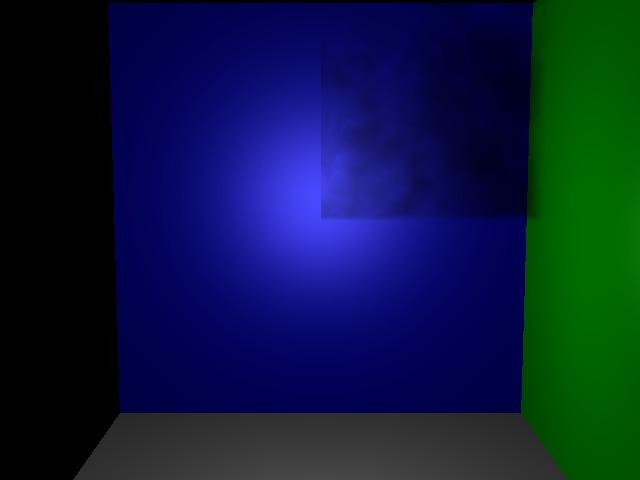
\includegraphics[scale=0.5]{no_scatter_abs020_scat090.jpg} \\
    \textbf{hit.scatter} = \textbf{(0,0,0)} et $\sigma_a$ = 0.2 et $\sigma_s$ = 0.9
\end{center}
\begin{center}
    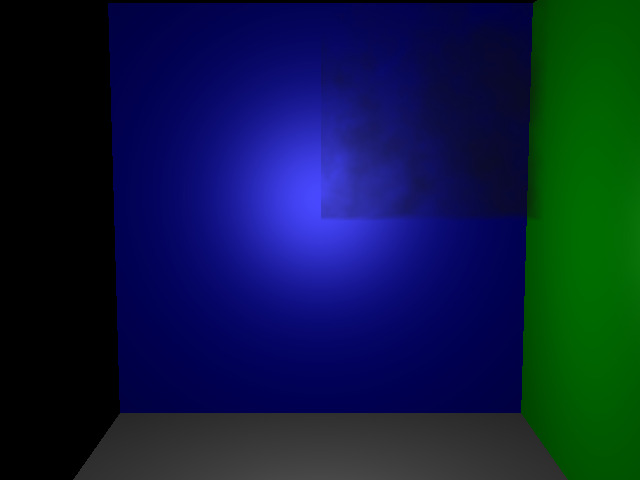
\includegraphics[scale=0.5]{scatter_abs020_scat090.jpg} \\
    \textbf{hit.scatter} $\neq$ \textbf{(0,0,0)} et $\sigma_a$ = 0.2 et $\sigma_s$ = 0.9
\end{center}
À première vue, la différence est difficile à remarquer, cependant elle est tout de même présente. La plus grande différence est la couleur de la fumée. Dans le coin en haut à droite, dans la première image, la fumée est considérablement plus foncée que dans la seconde. \\\\
De plus, j'ai finalement implémenté du bruit de perlin pour générer les densités dans mes voxels. Le résultat est une fumée plus réaliste qu'avant. \\\\
Ensuite, j'ai implémenter les autres types de \textbf{Ray Marcher} (Pas régulier, Pas régulier avec jitter, Centre du voxel, Centre du voxel avec jitter). \\\\
En ce moment, je travaille sur une nouvelle fonction de \textbf{Shading} pour pouvoir faire en sorte que le volume de fumée produise des ombres sur les objets de la scène. En ce moment, la fonction de \textbf{shading} est binaire. Soit que l'objet reçoit de la lumière, soit il n'en reçoit pas. La différence avec la fumée est que l'objet peut recevoir 50\% (par exemple) de la lumière plutôt que juste 0\% ou 100\%. Malgré le fait que le changement ne semble pas si compliqué que ça, je n'ai pas encore été en mesure d'obtenir des résultats convaincants, alors mon objectif pour le moment est d'avoir un bon \textbf{Shadinfg}.
\end{document}